\documentclass[twoside]{book}

% Packages required by doxygen
\usepackage{calc}
\usepackage{doxygen}
\usepackage{graphicx}
\usepackage[utf8]{inputenc}
\usepackage{makeidx}
\usepackage{multicol}
\usepackage{multirow}
\usepackage{fixltx2e}
\PassOptionsToPackage{warn}{textcomp}
\usepackage{textcomp}
\usepackage[nointegrals]{wasysym}
\usepackage[table]{xcolor}

% Font selection
\usepackage[T1]{fontenc}
\usepackage{mathptmx}
\usepackage[scaled=.90]{helvet}
\usepackage{courier}
\usepackage{amssymb}
\usepackage{sectsty}
\renewcommand{\familydefault}{\sfdefault}
\allsectionsfont{%
  \fontseries{bc}\selectfont%
  \color{darkgray}%
}
\renewcommand{\DoxyLabelFont}{%
  \fontseries{bc}\selectfont%
  \color{darkgray}%
}
\newcommand{\+}{\discretionary{\mbox{\scriptsize$\hookleftarrow$}}{}{}}

% Page & text layout
\usepackage{geometry}
\geometry{%
  a4paper,%
  top=2.5cm,%
  bottom=2.5cm,%
  left=2.5cm,%
  right=2.5cm%
}
\tolerance=750
\hfuzz=15pt
\hbadness=750
\setlength{\emergencystretch}{15pt}
\setlength{\parindent}{0cm}
\setlength{\parskip}{0.2cm}
\makeatletter
\renewcommand{\paragraph}{%
  \@startsection{paragraph}{4}{0ex}{-1.0ex}{1.0ex}{%
    \normalfont\normalsize\bfseries\SS@parafont%
  }%
}
\renewcommand{\subparagraph}{%
  \@startsection{subparagraph}{5}{0ex}{-1.0ex}{1.0ex}{%
    \normalfont\normalsize\bfseries\SS@subparafont%
  }%
}
\makeatother

% Headers & footers
\usepackage{fancyhdr}
\pagestyle{fancyplain}
\fancyhead[LE]{\fancyplain{}{\bfseries\thepage}}
\fancyhead[CE]{\fancyplain{}{}}
\fancyhead[RE]{\fancyplain{}{\bfseries\leftmark}}
\fancyhead[LO]{\fancyplain{}{\bfseries\rightmark}}
\fancyhead[CO]{\fancyplain{}{}}
\fancyhead[RO]{\fancyplain{}{\bfseries\thepage}}
\fancyfoot[LE]{\fancyplain{}{}}
\fancyfoot[CE]{\fancyplain{}{}}
\fancyfoot[RE]{\fancyplain{}{\bfseries\scriptsize Generated on Wed Dec 16 2015 13\+:07\+:32 for Project 2 by Doxygen }}
\fancyfoot[LO]{\fancyplain{}{\bfseries\scriptsize Generated on Wed Dec 16 2015 13\+:07\+:32 for Project 2 by Doxygen }}
\fancyfoot[CO]{\fancyplain{}{}}
\fancyfoot[RO]{\fancyplain{}{}}
\renewcommand{\footrulewidth}{0.4pt}
\renewcommand{\chaptermark}[1]{%
  \markboth{#1}{}%
}
\renewcommand{\sectionmark}[1]{%
  \markright{\thesection\ #1}%
}

% Indices & bibliography
\usepackage{natbib}
\usepackage[titles]{tocloft}
\setcounter{tocdepth}{3}
\setcounter{secnumdepth}{5}
\makeindex

% Hyperlinks (required, but should be loaded last)
\usepackage{ifpdf}
\ifpdf
  \usepackage[pdftex,pagebackref=true]{hyperref}
\else
  \usepackage[ps2pdf,pagebackref=true]{hyperref}
\fi
\hypersetup{%
  colorlinks=true,%
  linkcolor=blue,%
  citecolor=blue,%
  unicode%
}

% Custom commands
\newcommand{\clearemptydoublepage}{%
  \newpage{\pagestyle{empty}\cleardoublepage}%
}


%===== C O N T E N T S =====

\begin{document}

% Titlepage & ToC
\hypersetup{pageanchor=false,
             bookmarks=true,
             bookmarksnumbered=true,
             pdfencoding=unicode
            }
\pagenumbering{roman}
\begin{titlepage}
\vspace*{7cm}
\begin{center}%
{\Large Project 2 }\\
\vspace*{1cm}
{\large Generated by Doxygen 1.8.7}\\
\vspace*{0.5cm}
{\small Wed Dec 16 2015 13:07:32}\\
\end{center}
\end{titlepage}
\clearemptydoublepage
\tableofcontents
\clearemptydoublepage
\pagenumbering{arabic}
\hypersetup{pageanchor=true}

%--- Begin generated contents ---
\chapter{Hierarchical Index}
\section{Class Hierarchy}
This inheritance list is sorted roughly, but not completely, alphabetically\+:\begin{DoxyCompactList}
\item \contentsline{section}{Dice}{\pageref{class_dice}}{}
\begin{DoxyCompactList}
\item \contentsline{section}{Fancy\+Dice}{\pageref{class_fancy_dice}}{}
\end{DoxyCompactList}
\item \contentsline{section}{Throw\+Results}{\pageref{struct_throw_results}}{}
\item \contentsline{section}{User}{\pageref{struct_user}}{}
\item \contentsline{section}{Virtual\+Score}{\pageref{class_virtual_score}}{}
\begin{DoxyCompactList}
\item \contentsline{section}{Score}{\pageref{class_score}}{}
\end{DoxyCompactList}
\end{DoxyCompactList}

\chapter{Class Index}
\section{Class List}
Here are the classes, structs, unions and interfaces with brief descriptions\+:\begin{DoxyCompactList}
\item\contentsline{section}{\hyperlink{class_dice}{Dice} }{\pageref{class_dice}}{}
\item\contentsline{section}{\hyperlink{class_fancy_dice}{Fancy\+Dice} }{\pageref{class_fancy_dice}}{}
\item\contentsline{section}{\hyperlink{class_score}{Score} }{\pageref{class_score}}{}
\item\contentsline{section}{\hyperlink{struct_throw_results}{Throw\+Results} }{\pageref{struct_throw_results}}{}
\item\contentsline{section}{\hyperlink{struct_user}{User} }{\pageref{struct_user}}{}
\item\contentsline{section}{\hyperlink{class_virtual_score}{Virtual\+Score} }{\pageref{class_virtual_score}}{}
\end{DoxyCompactList}

\chapter{Class Documentation}
\hypertarget{class_dice}{\section{Dice Class Reference}
\label{class_dice}\index{Dice@{Dice}}
}
Inheritance diagram for Dice\+:\begin{figure}[H]
\begin{center}
\leavevmode
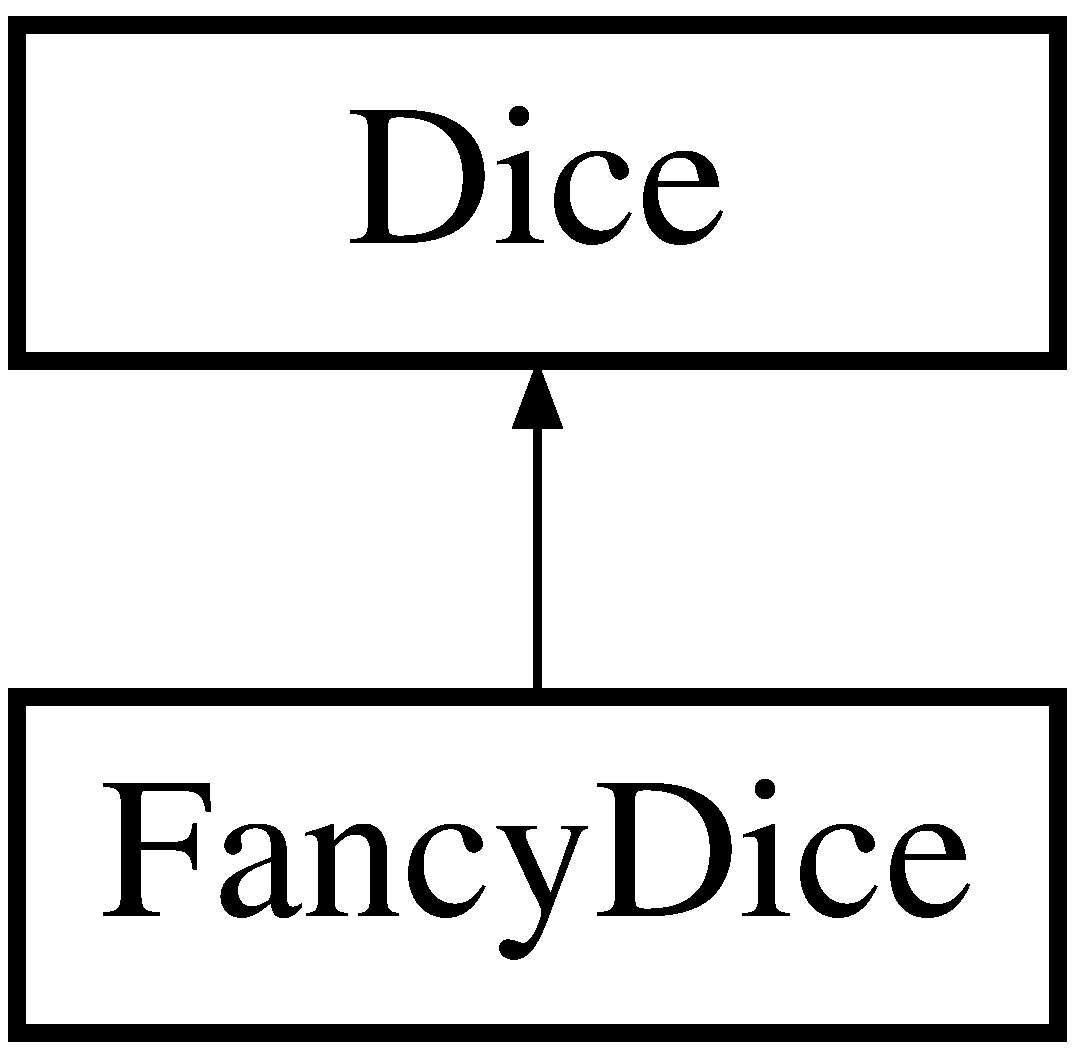
\includegraphics[height=2.000000cm]{class_dice}
\end{center}
\end{figure}
\subsection*{Public Member Functions}
\begin{DoxyCompactItemize}
\item 
\hypertarget{class_dice_a387ae2eb9925a0446dbe71ea2277e7c4}{void {\bfseries rolling} ()}\label{class_dice_a387ae2eb9925a0446dbe71ea2277e7c4}

\item 
\hypertarget{class_dice_a59e82d0bfe38167f094fc3db73cb409f}{void {\bfseries holding} ()}\label{class_dice_a59e82d0bfe38167f094fc3db73cb409f}

\end{DoxyCompactItemize}


The documentation for this class was generated from the following files\+:\begin{DoxyCompactItemize}
\item 
Dice.\+h\item 
Dice.\+cpp\end{DoxyCompactItemize}

\hypertarget{class_fancy_dice}{\section{Fancy\+Dice Class Reference}
\label{class_fancy_dice}\index{Fancy\+Dice@{Fancy\+Dice}}
}
Inheritance diagram for Fancy\+Dice\+:\begin{figure}[H]
\begin{center}
\leavevmode
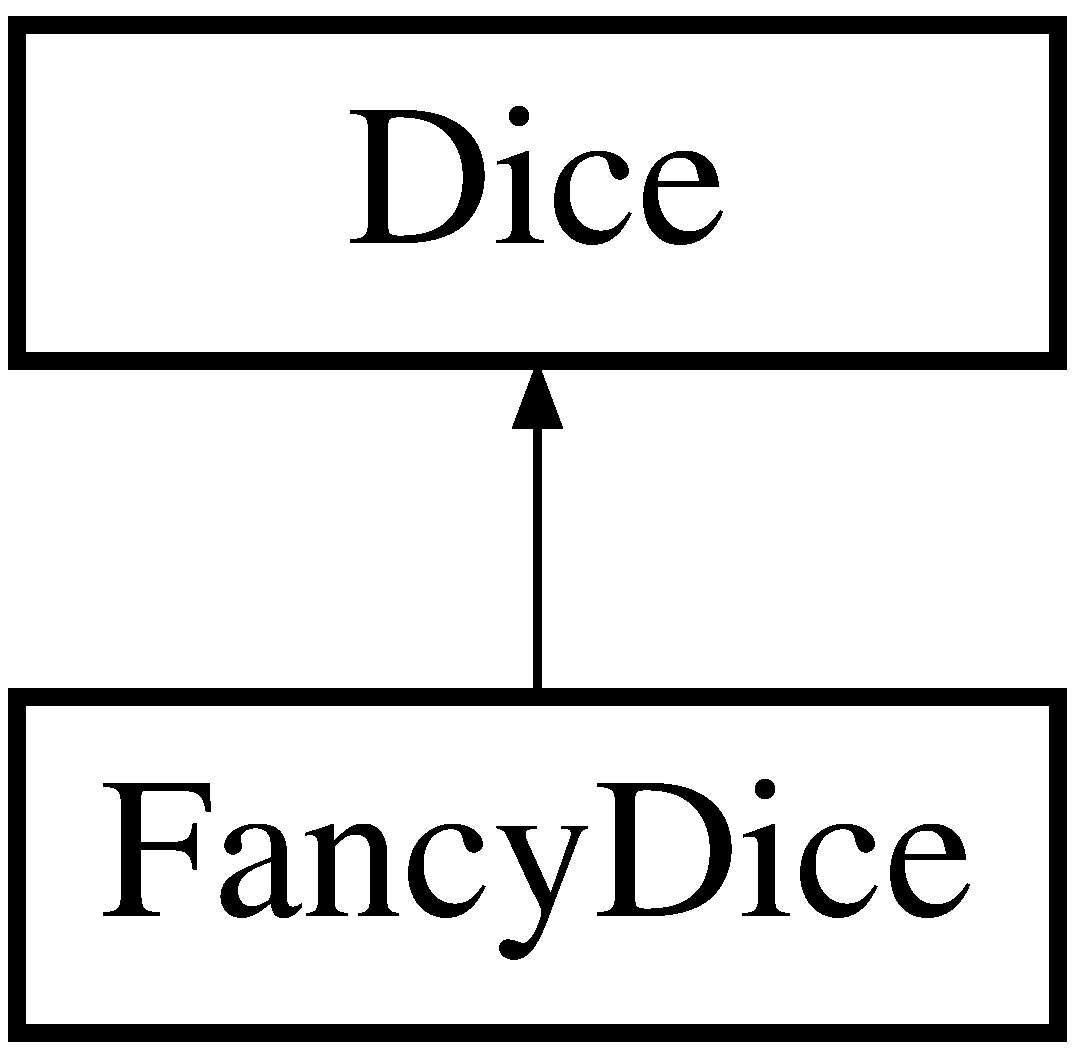
\includegraphics[height=2.000000cm]{class_fancy_dice}
\end{center}
\end{figure}
\subsection*{Public Member Functions}
\begin{DoxyCompactItemize}
\item 
\hypertarget{class_fancy_dice_aee1a0ad946b3a83693d61fdfefd15519}{void {\bfseries face1} ()}\label{class_fancy_dice_aee1a0ad946b3a83693d61fdfefd15519}

\item 
\hypertarget{class_fancy_dice_a30aa10cd3b5f645012f33e8e1531c9d9}{void {\bfseries face2} ()}\label{class_fancy_dice_a30aa10cd3b5f645012f33e8e1531c9d9}

\item 
\hypertarget{class_fancy_dice_ad6546af6fa0b63879717d7480367fe83}{void {\bfseries face3} ()}\label{class_fancy_dice_ad6546af6fa0b63879717d7480367fe83}

\item 
\hypertarget{class_fancy_dice_aa5bedabae1330f3fe52915906890c926}{void {\bfseries face4} ()}\label{class_fancy_dice_aa5bedabae1330f3fe52915906890c926}

\item 
\hypertarget{class_fancy_dice_a4de2b6d00791ad13a63c0c5c62d26ba8}{void {\bfseries face5} ()}\label{class_fancy_dice_a4de2b6d00791ad13a63c0c5c62d26ba8}

\item 
\hypertarget{class_fancy_dice_ae20e50b14a9e61fceefee7f12d18932e}{void {\bfseries face6} ()}\label{class_fancy_dice_ae20e50b14a9e61fceefee7f12d18932e}

\end{DoxyCompactItemize}


The documentation for this class was generated from the following files\+:\begin{DoxyCompactItemize}
\item 
Dice.\+h\item 
Dice.\+cpp\end{DoxyCompactItemize}

\hypertarget{class_score}{\section{Score Class Reference}
\label{class_score}\index{Score@{Score}}
}
Inheritance diagram for Score\+:\begin{figure}[H]
\begin{center}
\leavevmode
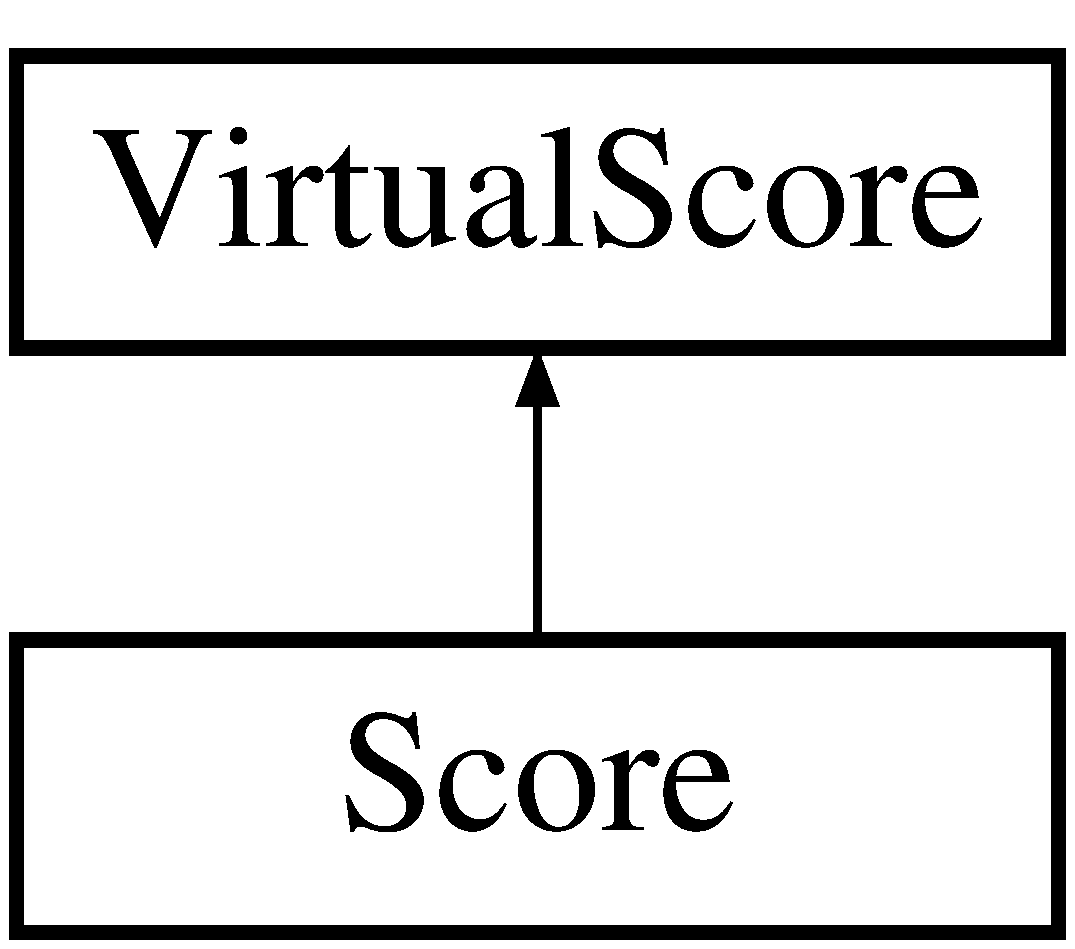
\includegraphics[height=2.000000cm]{class_score}
\end{center}
\end{figure}
\subsection*{Public Member Functions}
\begin{DoxyCompactItemize}
\item 
\hypertarget{class_score_a4cfb5cce9809de42f8bd08722705d674}{void {\bfseries score\+Board} (int potential\+Score, int over\+All\+Score)}\label{class_score_a4cfb5cce9809de42f8bd08722705d674}

\item 
\hypertarget{class_score_a8aa717c5b5dd793d256a2b78ae40573f}{void {\bfseries comp\+Score\+Board} (int potenital\+Score, int comp\+Overall\+Score)}\label{class_score_a8aa717c5b5dd793d256a2b78ae40573f}

\item 
\hypertarget{class_score_a28999bb14fa415da37c81bb7f7e102dc}{void {\bfseries clear\+Screen} (int potenital\+Score, int dice\+Score, int over\+All\+Score)}\label{class_score_a28999bb14fa415da37c81bb7f7e102dc}

\item 
\hypertarget{class_score_a4efe5d651d4a3a4db16423d0b4522180}{void {\bfseries comp\+Clear\+Screen} (int potential\+Score, int dice\+Score, int comp\+Overall\+Score)}\label{class_score_a4efe5d651d4a3a4db16423d0b4522180}

\end{DoxyCompactItemize}


The documentation for this class was generated from the following files\+:\begin{DoxyCompactItemize}
\item 
Score.\+h\item 
Score.\+cpp\end{DoxyCompactItemize}

\hypertarget{struct_throw_results}{\section{Throw\+Results Struct Reference}
\label{struct_throw_results}\index{Throw\+Results@{Throw\+Results}}
}
\subsection*{Public Attributes}
\begin{DoxyCompactItemize}
\item 
\hypertarget{struct_throw_results_adb1b2c3df923a0d475893660f5a02335}{float {\bfseries avg}}\label{struct_throw_results_adb1b2c3df923a0d475893660f5a02335}

\item 
\hypertarget{struct_throw_results_a5787e1fb78d5a40032987c03663e115d}{float {\bfseries median}}\label{struct_throw_results_a5787e1fb78d5a40032987c03663e115d}

\item 
\hypertarget{struct_throw_results_a59a84806bbe37cc26c50b908a16e05d3}{int $\ast$ {\bfseries mode}}\label{struct_throw_results_a59a84806bbe37cc26c50b908a16e05d3}

\item 
\hypertarget{struct_throw_results_a24bae5f8fce6933e2f6aa9e7f5ae4341}{int {\bfseries n\+Modes}}\label{struct_throw_results_a24bae5f8fce6933e2f6aa9e7f5ae4341}

\item 
\hypertarget{struct_throw_results_aeb6e628a45838285b3540de1d9b0a291}{int {\bfseries max\+Freq}}\label{struct_throw_results_aeb6e628a45838285b3540de1d9b0a291}

\end{DoxyCompactItemize}


The documentation for this struct was generated from the following file\+:\begin{DoxyCompactItemize}
\item 
main.\+cpp\end{DoxyCompactItemize}

\hypertarget{struct_user}{\section{User Struct Reference}
\label{struct_user}\index{User@{User}}
}
\subsection*{Public Attributes}
\begin{DoxyCompactItemize}
\item 
\hypertarget{struct_user_a643f85779a4693855c171c396f49e515}{string {\bfseries name}}\label{struct_user_a643f85779a4693855c171c396f49e515}

\item 
\hypertarget{struct_user_aa5829689588d1f982e1a69b73bd68655}{int {\bfseries age}}\label{struct_user_aa5829689588d1f982e1a69b73bd68655}

\item 
\hypertarget{struct_user_abffed56e4aa12d18466d6afc0c33be92}{string {\bfseries race}}\label{struct_user_abffed56e4aa12d18466d6afc0c33be92}

\item 
\hypertarget{struct_user_ac6d672a782dd5e58dd015b1c162eaf56}{string {\bfseries gender}}\label{struct_user_ac6d672a782dd5e58dd015b1c162eaf56}

\item 
\hypertarget{struct_user_ae83ced5dcd5903bf1851db48df97c179}{Day {\bfseries favorite\+Day}}\label{struct_user_ae83ced5dcd5903bf1851db48df97c179}

\item 
\hypertarget{struct_user_aa87d6def0ea86de58f7badf9512935c3}{bool {\bfseries pass}}\label{struct_user_aa87d6def0ea86de58f7badf9512935c3}

\end{DoxyCompactItemize}


The documentation for this struct was generated from the following file\+:\begin{DoxyCompactItemize}
\item 
main.\+cpp\end{DoxyCompactItemize}

\hypertarget{class_virtual_score}{\section{Virtual\+Score Class Reference}
\label{class_virtual_score}\index{Virtual\+Score@{Virtual\+Score}}
}
Inheritance diagram for Virtual\+Score\+:\begin{figure}[H]
\begin{center}
\leavevmode
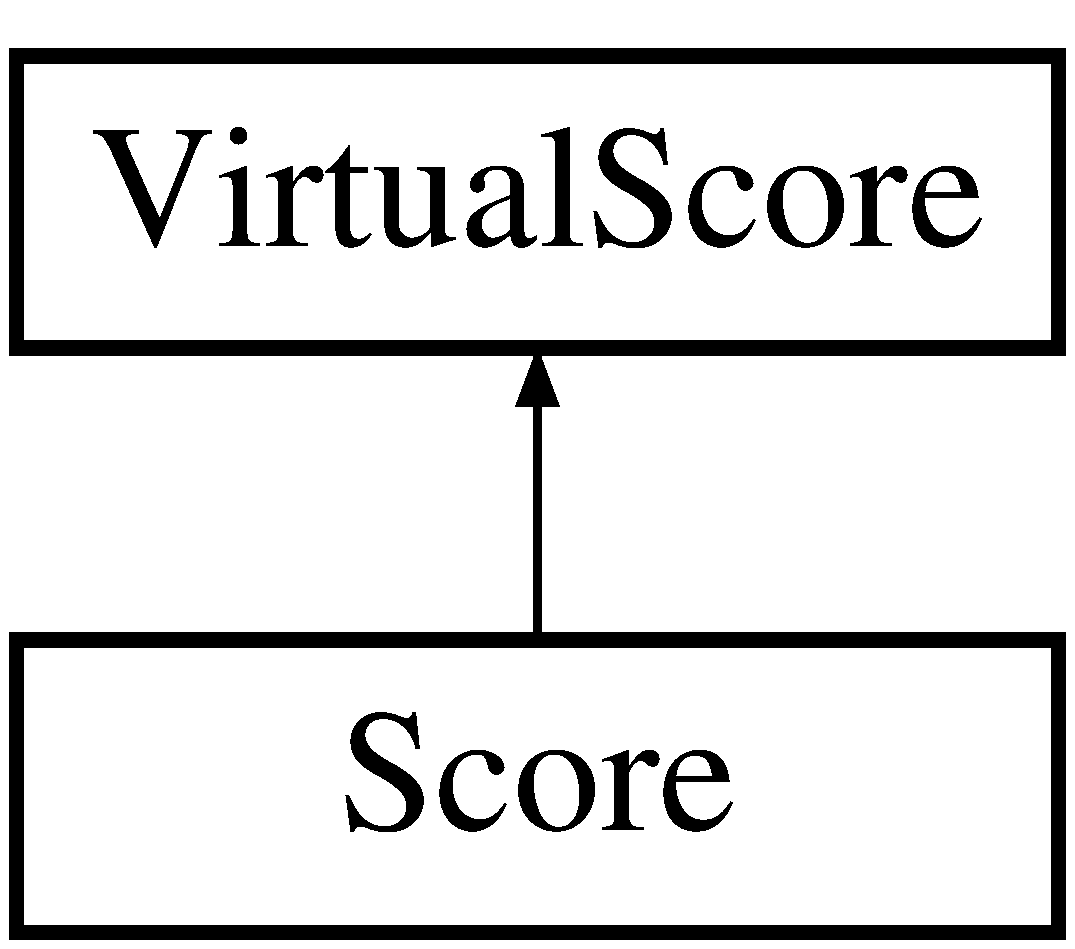
\includegraphics[height=2.000000cm]{class_virtual_score}
\end{center}
\end{figure}


The documentation for this class was generated from the following file\+:\begin{DoxyCompactItemize}
\item 
Score.\+h\end{DoxyCompactItemize}

%--- End generated contents ---

% Index
\newpage
\phantomsection
\addcontentsline{toc}{chapter}{Index}
\printindex

\end{document}
